\documentclass[compress]{beamer}
\usepackage{ifthen,verbatim}

\setbeamertemplate{navigation symbols}{}

\newcommand{\isnote}{}
\xdefinecolor{lightyellow}{rgb}{1.,1.,0.25}
\xdefinecolor{darkblue}{rgb}{0.1,0.1,0.7}

\begin{document}
\begin{frame}
\frametitle{CRAFT09 CSC track-based alignment}

\begin{itemize}
\item Chamber misalignment is smaller than misalignment of the disks they're mounted on
\item Diagnostic plot for ME$+$1/1: $r\phi$ residuals (mm) versus $\phi$
  from $-\pi$ to $\pi$, with smaller binning than chamber widths

  {\scriptsize \textcolor{darkblue}{Shades of} \textcolor{blue}{blue} are 2-D histogram, black points are profile, \textcolor{red}{red curve} is disk-fit, dashed lines are the chamber boundaries}

\item Fit $\delta_x\sin\phi+\delta_y\cos\phi+\delta_{\phi_z}$ for position {\scriptsize ($\delta_x$, $\delta_y$)} and angle {\scriptsize ($\delta_{\phi_z}$)}

  {\scriptsize ME$+$1/1: $\delta_x = 4.7 \pm 0.1$~mm, $\delta_y = 1.2 \pm 0.1$~mm, $\delta_{\phi_z} = -0.11 \pm 0.04$~mrad}
\end{itemize}

\mbox{\hspace{-1 cm}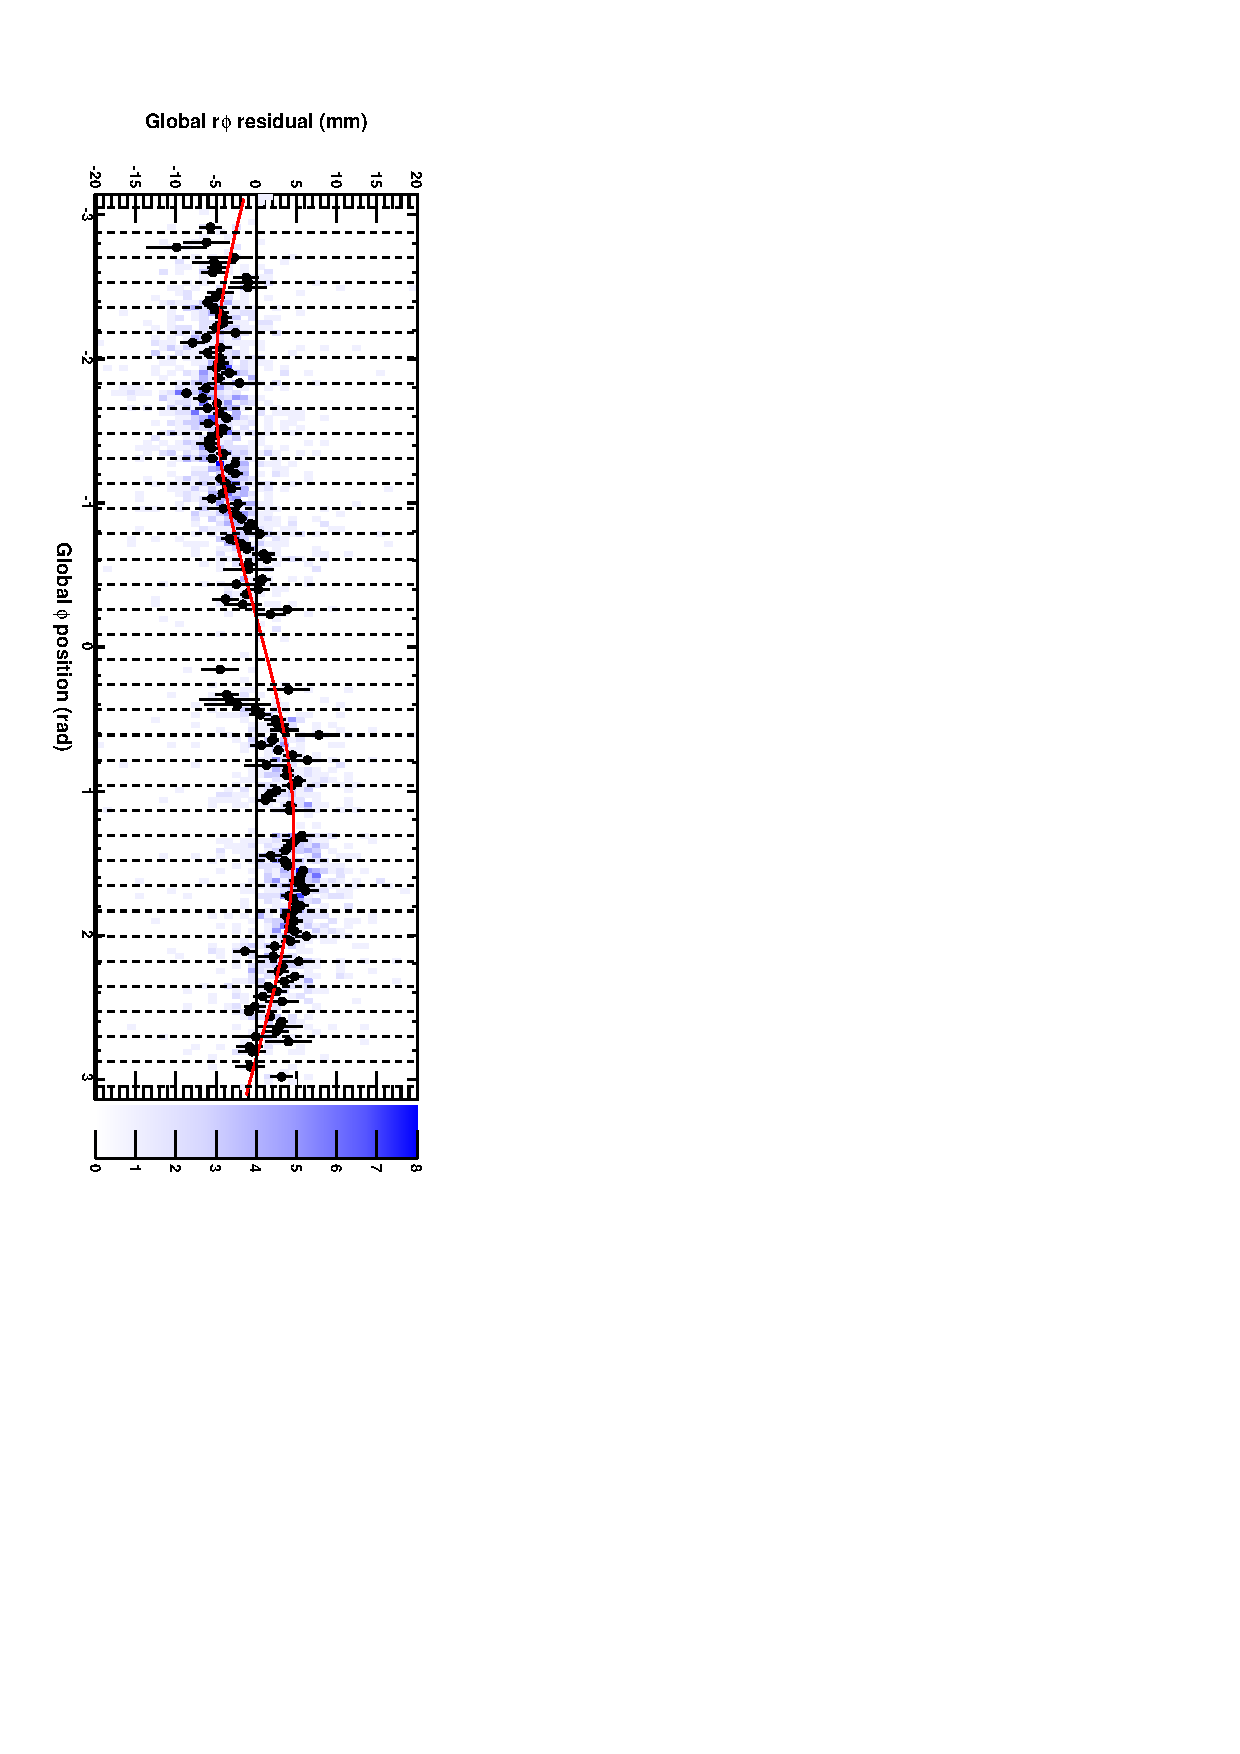
\includegraphics[height=1.2\linewidth, angle=90]{demonstrate_2009.pdf}}
\end{frame}

\end{document}
